\documentclass[12pt, letterpaper, titlepage]{article}

\usepackage{amsmath}
\usepackage{booktabs}
\usepackage{amsthm}
\usepackage{graphicx}
\usepackage[margin=1in]{geometry}
\usepackage{hyperref, url}
\hypersetup{colorlinks = true, linkcolor = blue, citecolor=blue, urlcolor = blue}
\usepackage{natbib}
\usepackage{enumitem}
\usepackage{setspace}

\usepackage[pagewise]{lineno}
%\linenumbers*[1]
% %% patches to make lineno work better with amsmath
\newcommand*\patchAmsMathEnvironmentForLineno[1]{%
 \expandafter\let\csname old#1\expandafter\endcsname\csname #1\endcsname
 \expandafter\let\csname oldend#1\expandafter\endcsname\csname end#1\endcsname
 \renewenvironment{#1}%
 {\linenomath\csname old#1\endcsname}%
 {\csname oldend#1\endcsname\endlinenomath}}%
\newcommand*\patchBothAmsMathEnvironmentsForLineno[1]{%
 \patchAmsMathEnvironmentForLineno{#1}%
 \patchAmsMathEnvironmentForLineno{#1*}}%

\AtBeginDocument{%
 \patchBothAmsMathEnvironmentsForLineno{equation}%
 \patchBothAmsMathEnvironmentsForLineno{align}%
 \patchBothAmsMathEnvironmentsForLineno{flalign}%
 \patchBothAmsMathEnvironmentsForLineno{alignat}%
 \patchBothAmsMathEnvironmentsForLineno{gather}%
 \patchBothAmsMathEnvironmentsForLineno{multline}%
}

% control floats
\renewcommand\floatpagefraction{.9}
\renewcommand\topfraction{.9}
\renewcommand\bottomfraction{.9}
\renewcommand\textfraction{.1}
\setcounter{totalnumber}{50}
\setcounter{topnumber}{50}
\setcounter{bottomnumber}{50}

\newcommand{\jy}[1]{\textcolor{blue}{JY: #1}}
\newcommand{\eds}[1]{\textcolor{red}{EDS: (#1)}}


\title{Sample Length at Which Block Bootstrapping is Effective for Estimation of Parameter of Time Series}

\author{Mathew Chandy\\
%   \href{mailto:mathew.chandy@uconn.edu}
% {\nolinkurl{mathew.chandy@uconn.edu}}\\
  Jun Yan\\[1ex]
  Department of Statistics, University of Connecticut\\
}
\date{}

\begin{document} 
\maketitle

\doublespace

\begin{abstract}
Block bootstrap is a method that is useful for estimating a parameter of a time
series. Theoretically, the method will work perfectly given an infinitely large sample of the time series.
It is necessary to know how large of a finite sample is required to for block bootstrap estimation to work. 
Before this study, there have been no investigations into this problem in the literature. The aim of this study 
is to answer this question by simulating replications of block bootstrap interval estimations of a parameter of a time series, 
and recording the rate at which the parameter is recovered by each replicate interval. 
The sample length required for acceptable performance is unsurprisingly found to be dependent 
on the type of interval construction and the series' level of temporal dependence.


\bigskip
\noindent\sc{Keywords}:
simulation;
\end{abstract}


\jy{Practice my writing tips on latex (e.g., keep line width under 80; use
  double blank lines to separate paragraphs; etc.):
  \url{https://statds.github.io/stat-writing/using-the-right-tools-for-writing.html}}

\jy{turn on the column number mode of your editor. Keep the width to under 80.}

\section{Introduction}
\label{sec:intro}

Block bootstrap is an important tool for constructing confidence intervals when
making inferences about dependent data. Early ideas were developed independently
by \citet{hall1985resampling}, \citet{carlstein1986use}, and 
\citet{kunsch1989jackknife}. % \citet{radovanov2014comparison}
It has been applied to a variety of different domains such 
as econometrics \citep{mackinnon2006bootstrap} and meteorology
\citep{varga2017generalised}. It is particularly useful for serially dependent
data when the serial dependence is not specified or of not primary interest.
As the sample size goes to infinity, block bootstrap confidence intervals are
expected to have coverage rates matching their nominal levels. For finite sample
sizes, however, a natural question is, how large a sample size is large enough
for block bootstrap confidence intervals to have the desired coverage rates?


\citet{hesterberg2015teachers} notes that while percentile-based confidence intervals from basic nonparametric bootstrap 
(simple resampling with no blocks involved) are more accurate than t-intervals for larger sample sizes, 
they are less accurate for smaller sample sizes. \citet{nevitt2001performance} find that a sample size of 
200-1000 is usually sufficient for interval estimation using basic nonparametric bootstrap.
\citet{goncalves2005bootstrap} found that standard error estimates from block bootstrap small 
samples may be significantly more accurate than inference from closed-form asymptotic estimates. 
That study focused on the estimation of a coefficient parameter within the context of linear regression. 
Still, the block bootstrap percentile confidence intervals under-covered the parameter even for n = 1024. 


While the aforementioned studies have looked into the necessary sample size for various bootstrap methods, 
the goal of this study is to find a threshold or range of sample sizes at which block bootstrap 
is an effective method for estimating a parameter specifically in the context of a time series. 
The method can be considered effective if approximately 1 - $\alpha$/2 \% of 1 - $\alpha$/2 \% of confidence intervals 
created from samples of the same size recover the parameter. This study will focus on estimating parameters of an 
AR(1) process with two types of block bootstrap confidence intervals from the literature, \citep{diciccio1996bootstrap}  \citep{rice2006mathematical} 
which is reviewed in Section 2. Section 3 offers an explanation of the simulation design and results. 
Section 4 discusses the results and how these findings could be useful.


\section{Review of Block Bootstrap}
\label{sec:blkbootreview}

Block bootstrap is a method that can be used to estimate a parameter of serially dependent data. Suppose that one wants to 
estimate a parameter or parameters $\theta$ of a population. The first step is to generate a sample of length $n$ from the population. 
An estimate of the parameter $\hat{\theta}_{n}$ can be computed from this sample. A pseudo-estimate $\hat\theta_n^*$ 
can be computed from a bootstrapped pseudo-sample. The mean $\bar\theta_n^*$ of many replicate $\hat\theta_n^*$ 
can also be computed. Lastly, for each $\hat\theta_n^*$, $\delta^* = \hat\theta_n^* - \bar\theta_n^*$ can be computed.


In basic bootstrap procedure, the new pseudo-sample of size $n$ would be created by simply resampling observations from 
the original sample with replacement. However, in the case of a time series, in order to account for the temporal dependence, 
the time series can be split into blocks, typically of the same size. The block should be of size $l$ large enough for each pseudo-sample
 to exhibit some temporal dependence, yet small enough for there to be some variability between each pseudo-sample. 
 Ideally, as $n$ increases, $l$ should also increase, but $l / n$ should decrease. To achieve this, $l$ is often assigned 
 a value as a function of $n$. A common function that is considered the best by much previous literature is 
 $l = \lceil n^{1/3} \rceil$ \citep{buhlmann1999block}. 
 The designer of the study can choose whether the blocks overlap or not. If the blocks do not overlap, it is called a non-moving block bootstrap. 
 In this case, the original sample is split evenly into blocks, which will then be resampled to create new pseudo-samples. 
 If the blocks do overlap, it is called a moving block bootstrap. Blocks are resampled randomly from the original sample, 
 but they do not have to be from a set of evenly spaced blocks. For moving block bootstrap, if $l \vert n$, a bootstrapped 
 pseudo-sample is created by taking a sample of $n / l$ blocks of size $l$ with replacement to create a new pseudo-sample of size $n$. 
 If $l does not divide n$, the pseudo-sample is created by taking a sample of $\lfloor n / l \rfloor$ blocks of size $l$ 
 and one block of size $(n \;\mathrm{mod})\; l$. An estimate $\hat\theta_n^*$ is computed from the pseudo-sample. 
 This procedure can be repeated many times to create a distribution of $\hat\theta_n^*$. 


In this study, 1000 $\hat\theta_n^*$ were created for one simulation of block bootstrap estimation. Using this distribution of 
$\hat\theta_n^*$, a $1 - \alpha$/2 \% confidence interval for the parameter can be constructed. 
The most simplistic method for constructing this interval is the percentile confidence interval. 
For a parameter $\theta$, the percentile $1 - \alpha$/2 \% confidence interval takes the form: 
\[ [\hat\theta_{n, \alpha/2}^*, \hat\theta_{n, 1 - \alpha/2}^*].\] 
Another method is the bias-corrected and accelerated 
(BCA) $1 - \alpha$/2 \% confidence interval, which takes the form: 
\[ [\hat\theta_{n, \alpha_1}^*,\hat\theta_{n, \alpha_2}^*].\] 
$\alpha_{1}$ and $\alpha_{2}$ are the cumulative probability of $z_{1}$ and $z_{2}$, respectively, where:
\[z_{1} = \frac{z_{0} - z_{1 - \alpha/2}}{1 - a(z_{0} - z_{1 - \alpha/2})} + z_{0}\] and
\[z_{2} = \frac{z_{0} + z_{1 - \alpha/2}}{1 - a(z_{0} + z_{1 - \alpha/2})} + z_{0}.\] 
Where $z_0$ is the quantile function of the proportion of $\hat\theta_n^* < \bar\theta_n^*$, 
and $a$ is the skewness of $\hat{\theta}_{n, -i}$, where $\hat{\theta}_{n, -i}$ is the statistic of the original sample computed without the $i^{th}$ block.
	
	
Both of these intervals work well when attempting to recover the mean and standard deviation of a temporally dependent process, 
but their coverage of the temporal dependence deteriorates as $n$ increases. A potential solution to this issue is to center the intervals 
$\hat{\theta}_{n}$. To do this, the distribution $\delta^*$ should be considered. A percentile interval 
centered around $\hat{\theta}_{n}$ ($CI_{\hat{\theta}_{n}}$) takes the form:
\[ [\hat{\theta}_{n} + \delta^*_{\alpha/2}, \hat{\theta}_{n} + \delta^*_{1 - \alpha/2}].\] 

%A percentile interval centered around $\bar\theta_n^*$ ($CI_{\bar\theta_n^*}$) takes the form: \[ [\bar\theta_n^* + \delta_{\alpha/2}, \bar\theta_n^* + \delta_{1 - \alpha/2}].\] An alternative is an interval of the form: \[ [\hat{\theta}_{n} - \delta^*_{1 - \alpha/2}, \hat{\theta}_{n} - \delta^*_{\alpha/2}],\] which is equivalent to: \[ [\hat{\theta}_{n} + \bar\theta_n^*- \hat\theta_{n, \alpha/2}^*, \hat{\theta}_{n} + \bar\theta_n^* - \hat\theta_{n, 1 - \alpha/2}^*],\] and therefore is also equivalent to: \[ [\bar\theta_n^* - \delta_{1 - \alpha/2}, \bar\theta_n^*- \delta_{\alpha/2}].\] Thus, the interval ($CI_{\hat{\theta}_{n}, \bar\theta_n^*}$) is centered around both $\hat{\theta}_{n}$ and $\bar\theta_n^*$.

This centering procedure can also be applied to a BCA interval. A BCA interval centered around $\hat{\theta}_{n}$ ($CI_{BCA, \hat{\theta}_{n}}$) takes the form:
\[ [\hat{\theta}_{n} + \delta^*_{\alpha_1}, \hat{\theta}_{n} + \delta^*_{\alpha_2}].\] 
%A BCA interval centered around $\bar\theta_n^*$ ($CI_{BCA, \bar\theta_n^*}$) takes the form: \[ [\bar\theta_n^* + \delta_{\alpha_1}, \bar\theta_n^* + \delta_{\alpha_2}].\] An alternative (($CI_{BCA, \hat{\theta}_{n}, \bar\theta_n^*}$) is an interval of the form: \[ [\hat{\theta}_{n} - \delta^*_{\alpha_2}, \hat{\theta}_{n} - \delta^*_{\alpha_1}]\] 

Thus, there are two types of intervals that can be constructed for block bootstrap estimation in this study: 
$CI_{\hat{\theta}_{n}}$ and $CI_{BCA, \hat{\theta}_{n}}$. Note that both of these intervals are centered around $\hat{\theta}_{n}$ and asymmetric. 


\section{Simulation Study}
\label{sec:simstudy}

%The central objective of the study was to assess what sample size is necessary for the the block bootstrap method to estimate a parameter of an autoregressive process. The method will work better as the sample size goes to infinity, but the goal is to see what is the smallest sample size that is acceptable. The sample size is acceptable if many 1 - $\alpha$/2 confidence intervals for that sample size recover the parameter at a rate of 1 - $\alpha$/2 \%. In the previous section, the procedures for creating three types of confidence interval of a parameter using the block bootstrap method are described. 

%These procedures are applied to a simulation of an autoregressive integrated moving average (ARIMA) process to create three confidence interval of certain parameters (the mean, the AR(1) coefficient, the MA(1) coefficient, the standard deviation, etc.). 



Base R has a built in function arima.sim that allows one to simulate an AR(1) process, for which one can set the theoretical $\phi$. 
By default, the mean of the process $\mu$ is 0 and the standard deviation of the error term $\sigma_{\epsilon}$ is 1. 
For the purposes of this study, the standard deviation of the process $\sigma_{x}$ should be controlled at 1. 
The observations can be multiplied by $\sqrt{1 - \phi^2}$ so that the new theoretical $\sigma_{x}$ is equivalent to 1, as shown below:
\begin{align}
X_{t} &= \epsilon_{t} + \phi X_{t-1};\\
Var(X_{t}) &= Var(\epsilon_{t} + \phi X_{t-1});\\
\sigma^2_{x} &= \sigma^2_{\epsilon} + \phi^2 \sigma^2_{x};\\
\sigma^2_{x}(1 - \phi^2) &= 1;\\
\sigma_{x}\sqrt{1 - \phi^2} &= 1.
\end{align}

The experimental factor of this study was $\phi$, as the temporal dependence affects the performance of block bootstrap. 
$\phi = -0.4 -0.2,$ and $0$ (a standard normal distribution)$, 0.2, and 0.4$ were used in this study. 


As described in the last section, the block bootstrap method can be used to estimate a parameter $\theta$ of an AR(1) process. 
This method can be simulated with the tsboot function from the boot R package. In this study, $\theta$ is composed of the target 
parameters $\mu = 0$, $\sigma_{x}$, and $\phi$. From a sample of length $n$, two types of block bootstrap 95\% confidence intervals 
can be constructed for each target parameter: $CI_{\hat{\theta}_{n}}$ and $CI_{BCA, \hat{\theta}_{n}}$.


Each of these 6 intervals either recovers $\theta$ or does not. Remember that 95\% of many of a certain type of 95\% confidence intervals 
constructed from samples of the same $n$ should recover $\theta$. To see if this is generally or approximately the case, one can run 
1000 replications of the block bootstrap procedure, and for each interval-$\theta$ pair, the rate at which that type of interval recovers 
$\theta$ can be recorded. The coverage rate is, of course, a point estimate of a proportion, so a 95\% confidence interval of this coverage proportion 
(with $n_{CI} = 1000$) can be constructed, and if the proportion .95 is included in the interval, the block bootstrap method is likely working well.


If $\theta$ is not covered at that $n$, a larger sample size must be necessary. $n = $100, 200, 300, 400, and 500, 600, 700 were used in this study. 
Remember that the goal is to find the smallest $n$ which is sufficient for proper coverage. 

%For all simulation studies, but $\mu$ and $\sigma_{x}$ can be kept constant, but increasing temporal dependence factors such as AR and MA Coefficients can make block bootstrap less effective in estimation, so its impact on the method's performance should be analyzed. For a certain variation of an AR(1) process, block bootstrap 95\% confidence intervals for each of 3 parameters ($\mu$, $\sigma_{x}$, and the autocorrelation function$\rho$) can be replicated for 1000 simulated samples of a certain length. For each individual confidence interval, it can be recorded whether or not the interval includes the true parameter. The coverage rate, or the proportion of intervals that include the true parameter, can then be recorded. If the parameter is being properly estimated by the block bootstrap, the coverage rate should reflect this by being close to the confidence level of 95\%. If this is not the case, the method is not working as well as it should. The width of the confidence interval for each replication is dependent on the variability of the parameter of the time series. If the interval is on average not wide enough to capture the parameter at the expected rate of 95\%, it indicates that the variability of the parameter is underestimated. If the interval is too wide and captures the parameter at a rate above 95\%, it indicates that the variability of the parameter is overestimated. Since the coverage rate is a proportion based on 1000 independent binary outcomes (the interval recovers the parameter or it doesn't), a 95\% confidence interval of the coverage rate for each parameter can also be created. The inclusion of .95 in the interval indicates that the block bootstrap method is working well for its respective parameter. If this is not the case for this sample length, the procedure can be conducted again with a larger sample length. This can be repeated until the method is determined to be working acceptably, meaning that .95 is included in the 95\% confidence interval of the coverage rate of the parameter.



%1000 replicates of length-n random samples of an AR(1) process with theoretical $\mu$ = 0, $\sigma_{x}$ = 1, and $\theta$ = 0.1 were simulated using R. For each of three target parameters ($\mu$ = 0, $\sigma_{x}$ = 1, and $\theta$ = 0.1, three types of block bootstrap (with block length l) confidence intervals (percentile, empirical, and BCA) were constructed for each replicate sample. The statistic used to estimate $\mu$ is the sample mean $\bar{x}$, the statistic used to estimate $\sigma$ is the sample standard deviation $S^2$, and the statistic used to estimate $\theta$ is the auto-correlation function of the sample. For each of these nine categories of confidence intervals, the coverage rate of its respective parameter was computed, along with a 95\% confidence interval of the proportion given 4000 trials. For a certain variation of the process, the study was repeated for n = 125, 1000, 3375, and 8000. The only parameter of the process that was varied was $\theta$, and 0.1, 0.3, and 0.5 were the values used.



\begin{figure}[tbp]
  \centering
  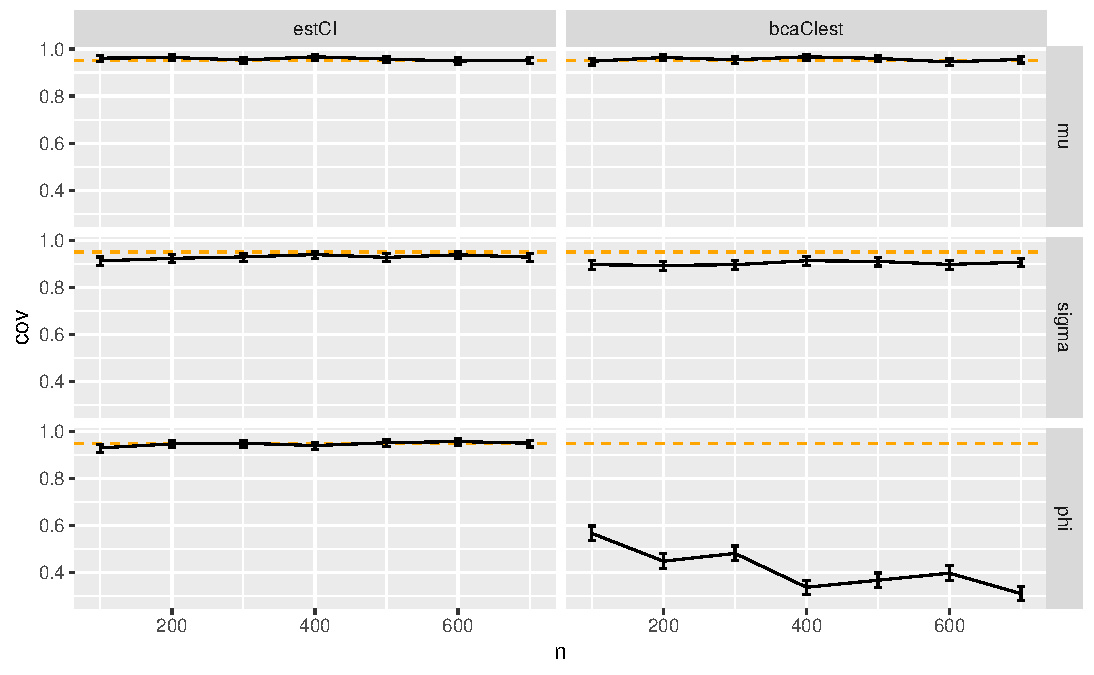
\includegraphics[width=\textwidth]{figures/plot_n.4}
  \caption{At $\phi = -.4$, both intervals covered $\mu$ correctly as low as $n = 100$. $CI_{\hat{\theta}_{n}}$ seems to cover $\sigma$ well as 
  low as $n = 400$. $CI_{BCA, \hat{\theta}_{n}}$ under-covers $\sigma$, but there is no clear pattern of deterioration of coverage, so one can 
  expect that increasing $n$ will eventually result in proper coverage of $\sigma$. $CI_{\hat{\theta}_{n}}$ covers $\phi$ well with no deterioration, 
  and this is true as low as $n = 200$. $CI_{BCA, \hat{\theta}_{n}}$ greatly under-covers $\phi$, and there is a clear pattern of deterioration of coverage.}
  \label{fig:plot_n.4}
\end{figure}


\begin{figure}[tbp]
  \centering
  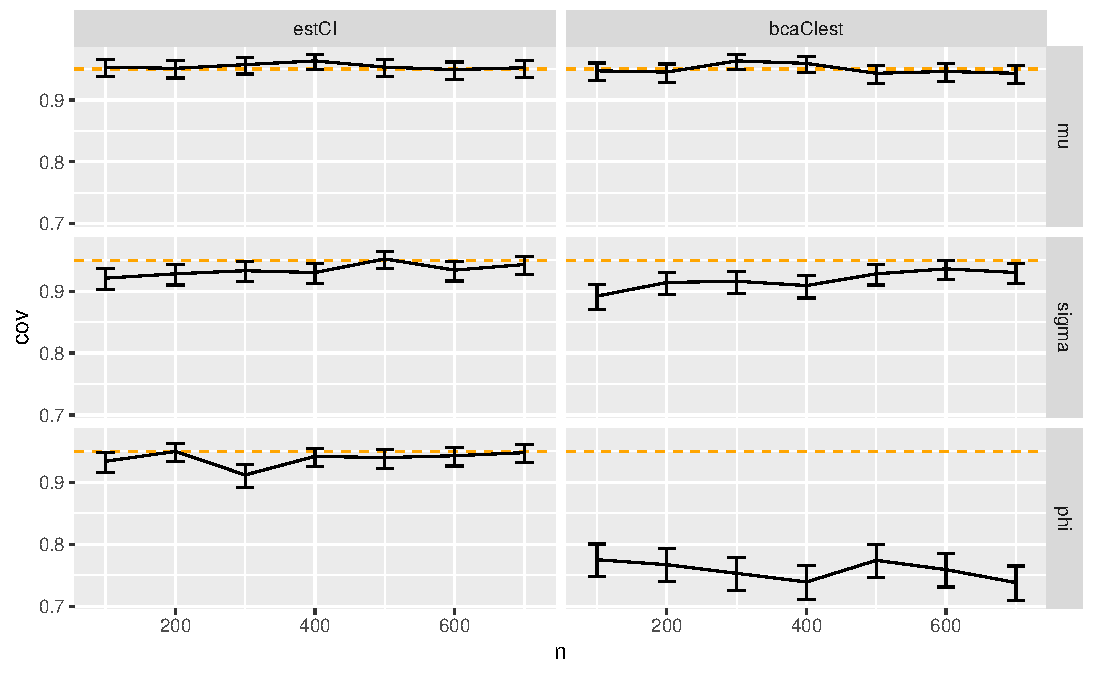
\includegraphics[width=\textwidth]{figures/plot_n.2}
  \caption{At $\phi = -.2$, both intervals covered $\mu$ correctly as low as $n = 100$. Both intervals seem to cover $\sigma$ generally well, 
  although $CI_{BCA, \hat{\theta}_{n}}$ has somewhat lower coverage rates. $CI_{\hat{\theta}_{n}}$ covers $\phi$ well with no deterioration of coverage, 
  and this is true as low as $n = 200$.  $CI_{BCA, \hat{\theta}_{n}}$ greatly under-covers $\phi$, and there is a clear coverage deterioration trend as $n$ increases.}
  \label{fig:plot_n.2}
\end{figure}


\begin{figure}[tbp]
  \centering
  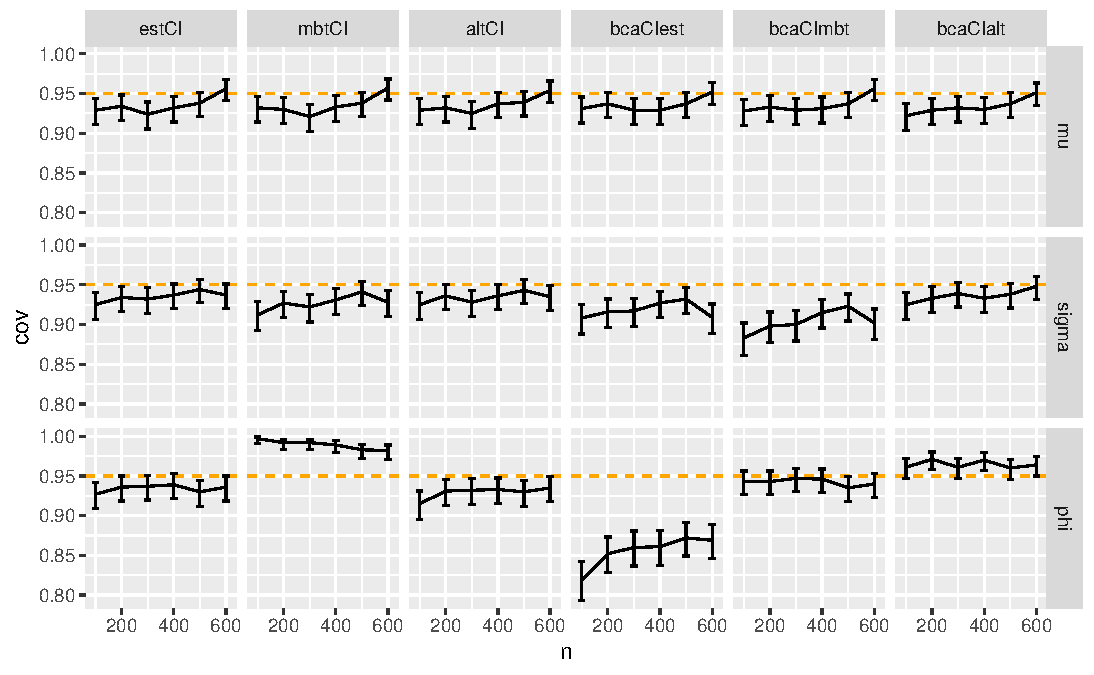
\includegraphics[width=\textwidth]{figures/plot_0}
  \caption{At $\phi = 0$, both intervals covered $\mu$ correctly as low as $n = 500$. $CI_{\hat{\theta}_{n}}$ seems to cover $\sigma$ well as low as 
  $n = 400$. $CI_{BCA, \hat{\theta}_{n}}$ slightly under-covers $\sigma$, but there is no clear pattern of deterioration of coverage, 
  so one can expect that increasing $n$ will eventually result in proper coverage of $\sigma$. $CI_{\hat{\theta}_{n}}$ seems to cover 
  $\phi$ generally well at $n = 400$, but $CI_{BCA, \hat{\theta}_{n}}$ under-covers $\phi$, although the method's performance seems to improve as $n$ increases.}
  \label{fig:plot_0}
\end{figure}

\begin{figure}[tbp]
  \centering
  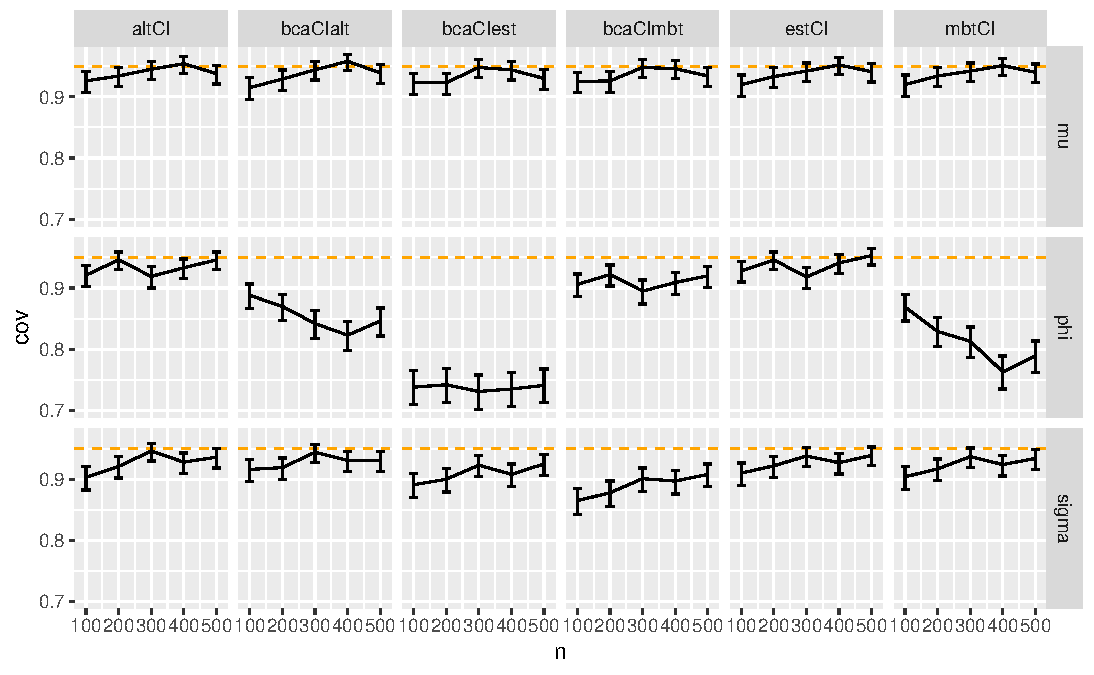
\includegraphics[width=\textwidth]{figures/plot_.2}
  \caption{At $\phi = .2$, both intervals covered $\mu$ correctly as low as $n = 300$. Both intervals seem to cover $\sigma$ generally well, 
  although $CI_{BCA, \hat{\theta}_{n}}$ has somewhat lower coverage rates. $CI_{\hat{\theta}_{n}}$ covers $\phi$ well with no deterioration of coverage, 
  and this is true as low as $n = 200$. $CI_{BCA, \hat{\theta}_{n}}$ greatly under-covers $\phi$, but there is no clear coverage deterioration trend as $n$ increases.}
  \label{fig:plot_.2}
\end{figure}

\begin{figure}[tbp]
  \centering
  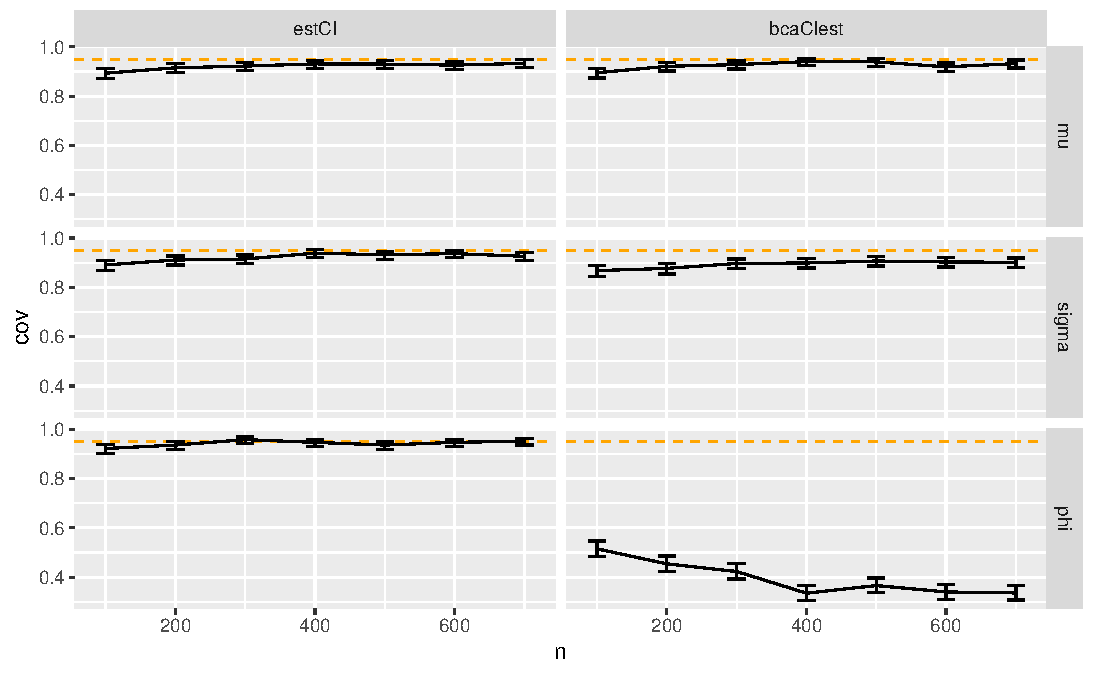
\includegraphics[width=\textwidth]{figures/plot_.4}
  \caption{At $\phi = .4$, both intervals seem to cover $\mu$ generally well as low as $n = 400$. $CI_{\hat{\theta}_{n}}$ 
  covers $\sigma$ well as low as $n = 400$. 
  $CI_{BCA, \hat{\theta}_{n}}$ under-covers $\sigma$, but there is no clear sign of coverage deterioration, so one can expect that 
  increasing $n$ 
  will eventually result in proper coverage of $\sigma$. $CI_{\hat{\theta}_{n}}$ covers $\phi$ well with no deterioration of coverage, 
  and this is true as low as $n = 200$. $CI_{BCA, \hat{\theta}_{n}}$ greatly under-covers $\phi$ with a clear coverage deterioration 
  trend as $n$ increases.}
  \label{fig:plot_.4}
\end{figure}


Only $CI_{\hat{\theta}_{n}}$ managed to solve the deterioration problem with respect to recovering $\phi$, indicating that this interval 
should be used as opposed to $CI_{BCA, \hat{\theta}_{n}}$ when estimating $\phi$. As expected, a higher $\phi$ demands a 
larger $n$ to estimate all parameters, but a negative $\phi$ may only require a lesser $n$. For example, for both $\phi = 0.2$ and $0.4$, 
$n = 100$ was sufficient to recover $\mu$ at a rate of approximately 95\%.

\section{Concluding Remarks}
\label{sec:conremarks}

The motivation for the study is the idea that block bootstrap procedure will perfectly estimate a parameter of a time series given 
an infinitely large sample. 
The goal for this study was to find what is a good enough finite sample length for block bootstrap estimation to recover 
the parameter of a 
time series at an acceptable rate. Assuming that $CI_{\hat{\theta}_{n}}$ is used (as it was found to work better overall, 
especially when estimation $\phi$), 
the results of this study suggest that even for estimating $\mu$, an $n$ of around 500 may be necessary if $\phi$ is unknown. 
An $n$ of around 400 may be necessary to estimate $\sigma$ is $\phi$ is unknown. If $\phi$ is already known, 
a lesser $n$ may be adequate to estimate these parameters. When $\phi$ was negative, 
a $n$ of around 100 was sufficient to estimate $\mu$. However, in real world applications, $\phi$ is more commonly found to be positive, 
so a larger $n$ is more likely to be necessary. Lastly, to estimate $\phi$, an $n$ of around 400 may be necessary. 
This information could prove to be useful for researching using block bootstrap estimation of time series in domains such as econometrics. 
Future studies could investigate if there are types of block bootstrap intervals that can be constructed that 
would more appropriate recover the parameters of a time series. One could also investigate the $n$ needed to 
make inferences about other forms of serially dependent data such as an MA process.


\bibliographystyle{chicago}
\bibliography{citations}[tp]

\end{document}

